\section{יחידה 11: בדיקת השערות סטטיסטיות}

יחידה זו עוסקת בבדיקת השערות לגבי פרמטרים באוכלוסייה,
על סמך מדגם מקרי, באמצעות התפלגות הדגימה.
זהו השימוש המרכזי בהתפלגות הדגימה של ממוצעים.



\subsection{הרעיון הכללי}

בדיקת השערות עונה על השאלה:
\begin{quote}
האם תוצאת המדגם סבירה בהנחה שטענה מסוימת על האוכלוסייה נכונה?
\end{quote}

הבדיקה אינה מוכיחה טענות, אלא בוחנת סבירות.



\subsection{השערות הבדיקה}

\subsubsection{השערת האפס $H_0$}
טענה שמרנית על האוכלוסייה, המניחה שאין אפקט או שאין שינוי.

\subsubsection{השערת המחקר $H_1$}
טענה חלופית, המייצגת אפקט, שינוי או כיוון מסוים.

\subsubsection{דגש למבחן}
הבדיקה מתבצעת תמיד \textbf{בהנחה ש־$H_0$ נכונה}.



\subsection{רמת המובהקות \texorpdfstring{$\alpha$}{α}}

\subsubsection{הגדרה}
ההסתברות לדחות את $H_0$ כאשר היא נכונה.

\subsubsection{פירוש אינטואיטיבי}
הסיכון שאנו מוכנים לקחת לטעות מסוג ראשון.

\subsubsection{ערכים נפוצים}
\[
\alpha = 0.05 \quad \text{או} \quad 0.01
\]



\subsection{סטטיסטי המבחן – מבחן Z}

כאשר סטיית התקן באוכלוסייה ידועה והתפלגות הדגימה נורמלית:

\[
Z = \frac{\bar{X} - \mu_0}{\sigma / \sqrt{n}}
\]

כאשר $\mu_0$ הוא הערך לפי $H_0$.

\subsubsection{מתי מותר להשתמש במבחן Z}

השימוש במבחן Z מבוסס על כך שסטטיסטי המבחן מתפלג בקירוב נורמלית.
דבר זה מתקיים כאשר לפחות אחד מהתנאים הבאים מתקיים:
\begin{itemize}
\item האוכלוסייה מתפלגת נורמלית
\item גודל המדגם גדול מספיק $(n \ge 30)$ – לפי משפט הגבול המרכזי
\end{itemize}

אם תנאים אלה אינם מתקיימים, הנחת הנורמליות אינה מוצדקת,
ומבחן Z אינו בהכרח תקף.
במקרה שהנחות אלו אינן מתקיימות,
יש להשתמש במבחן חלופי (כגון מבחן t).

\subsection{אזור דחייה וערך קריטי \texorpdfstring{$Z_c$}{Zc}}

אזור הערכים הקיצוניים של סטטיסטי המבחן, אשר הסתברותם קטנה מ־$\alpha$ בהנחת $H_0$. 

\subsubsection{1. בדיקה דו־צדדית (Two-tailed)}
נשתמש בה כאשר השערת המחקר היא לשינוי כלשהו $(H_1: \mu \neq \mu_0)$. 
אזור הדחייה מתחלק לשני הזנבות, כאשר בכל זנב יש שטח של $\alpha/2$.

\begin{figure}[H]
\centering
\begin{english}
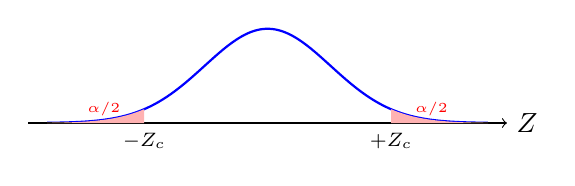
\begin{tikzpicture}[xscale=0.8, yscale=3]
  \draw[thick, blue, domain=-3.5:3.5, samples=150] plot (\x, {exp(-(\x*\x)/2)/sqrt(2*pi)});
  \draw[->] (-3.8,0) -- (3.8,0) node[right] {$Z$};
  \fill[red!30] (-3.5,0) -- plot[domain=-3.5:-1.96] (\x, {exp(-(\x*\x)/2)/sqrt(2*pi)}) -- (-1.96,0) -- cycle;
  \fill[red!30] (1.96,0) -- plot[domain=1.96:3.5] (\x, {exp(-(\x*\x)/2)/sqrt(2*pi)}) -- (3.5,0) -- cycle;
  \node[red] at (-2.6,0.06) {\tiny $\alpha/2$};
  \node[red] at (2.6,0.06) {\tiny $\alpha/2$};
  \node[below, font=\scriptsize] at (-1.96,0) {$-Z_c$};
  \node[below, font=\scriptsize] at (1.96,0) {$+Z_c$};
\end{tikzpicture}
\end{english}
\end{figure}

\subsubsection{2. בדיקה חד־צדדית ימנית (Right-tailed)}
נשתמש בה כאשר נשאלת שאלה על "עלייה" או "שיפור" $(H_1: \mu > \mu_0)$. 
כל שטח ה־$\alpha$ נמצא בזנב הימני.

\begin{figure}[H]
\centering
\begin{english}
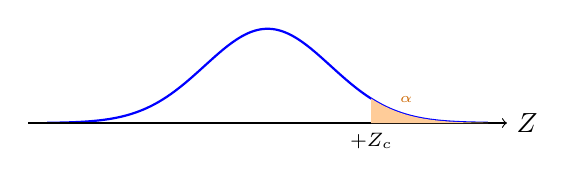
\begin{tikzpicture}[xscale=0.8, yscale=3]
  \draw[thick, blue, domain=-3.5:3.5, samples=150] plot (\x, {exp(-(\x*\x)/2)/sqrt(2*pi)});
  \draw[->] (-3.8,0) -- (3.8,0) node[right] {$Z$};
  \fill[orange!40] (1.645,0) -- plot[domain=1.645:3.5] (\x, {exp(-(\x*\x)/2)/sqrt(2*pi)}) -- (3.5,0) -- cycle;
  \node[orange!80!black] at (2.2,0.1) {\tiny $\alpha$};
  \node[below, font=\scriptsize] at (1.645,0) {$+Z_c$};
\end{tikzpicture}
\end{english}
\end{figure}

\subsubsection{3. בדיקה חד־צדדית שמאלית (Left-tailed)}
נשתמש בה כאשר נשאלת שאלה על "ירידה" או "הפחתה" $(H_1: \mu < \mu_0)$. 
כל שטח ה־$\alpha$ נמצא בזנב השמאלי.

\begin{figure}[H]
\centering
\begin{english}
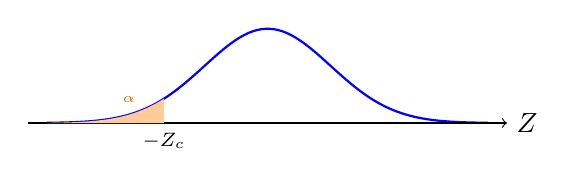
\begin{tikzpicture}[xscale=0.8, yscale=3]
  \draw[thick, blue, domain=-3.5:3.5, samples=150] plot (\x, {exp(-(\x*\x)/2)/sqrt(2*pi)});
  \draw[->] (-3.8,0) -- (3.8,0) node[right] {$Z$};
  \fill[orange!40] (-3.5,0) -- plot[domain=-3.5:-1.645] (\x, {exp(-(\x*\x)/2)/sqrt(2*pi)}) -- (-1.645,0) -- cycle;
  \node[orange!80!black] at (-2.2,0.1) {\tiny $\alpha$};
  \node[below, font=\scriptsize] at (-1.645,0) {$-Z_c$};
\end{tikzpicture}
\end{english}
\end{figure}

\subsection{p-value}

\subsubsection{הגדרה}
ההסתברות לקבל תוצאה קיצונית לפחות כמו התוצאה שנצפתה במדגם, בהנחה ש־$H_0$ נכונה.


\subsubsection{הקשר בין Z ל-p וחישובו}
קיים קשר הפוך בין המרחק של $Z$ מהמרכז לבין ה-$p$:
\begin{itemize}
    \item ככל שציון ה-Z המחושב רחוק יותר מהמרכז $\Longleftarrow$ ה-$p$ קטן יותר.
    \item אם ה-$Z$ המחושב גדול מה-$Z_c$ הקריטי $\Longleftarrow$ ה-$p$ בהכרח קטן מ-$\alpha$.
    \item \textbf{חישוב ה-p במבחן:}
    \begin{itemize}
        \item במבחן חד-צדדי: השטח בזנב מעבר ל-$Z$ שחישבנו (לפי טבלת ה-Z).
        \item במבחן דו-צדדי: השטח בזנב מעבר ל-$Z$ שחישבנו \textbf{כפול 2}.
    \end{itemize}
\end{itemize}

\subsubsection{כלל החלטה}
\begin{itemize}
\item אם $p \le \alpha$ – דוחים את $H_0$ (התוצאה מובהקת).
\item אם $p > \alpha$ – לא דוחים את $H_0$ (התוצאה אינה מובהקת).
\end{itemize}

\subsubsection{מה ה־p-value אינו}

\begin{itemize}
\item ה־$p$ אינו ההסתברות ש־$H_0$ נכונה
\item ה־$p$ אינו מדד לגודל האפקט
\item ה־$p$ אינו ההסתברות שטעינו
\end{itemize}

ה־$p$ מודד אך ורק את מידת הקיצוניות של הנתונים
בהנחה ש־$H_0$ נכונה.

\subsection{שלוש דרכי החלטה שקולות}

\begin{enumerate}
\item השוואת $Z$ לערך קריטי
\item השוואת $p$ ל־$\alpha$
\item בדיקה האם $\bar{X}$ נמצא באזור הדחייה
\end{enumerate}

כל הדרכים מובילות לאותה מסקנה.

\subsection{טעויות נפוצות}

\begin{itemize}
\item לחשוב ש־$p$ הוא ההסתברות ש־$H_0$ נכונה
\item לומר “מקבלים את $H_0$” במקום “לא דוחים”
\item לבחור חד/דו־צדדי אחרי ראיית הנתונים
\item לבלבל בין $\alpha$ ל־$p$
\end{itemize}

\subsection{פירוש ההחלטה הסטטיסטית}

\subsubsection{דחיית השערת האפס}
דחיית $H_0$ פירושה שהנתונים אינם סבירים בהנחתה,
ולכן קיימת עדות סטטיסטית לטובת $H_1$.

\subsubsection{אי־דחיית השערת האפס}
אי־דחיית $H_0$ אינה מוכיחה שהיא נכונה,
אלא רק שהנתונים אינם קיצוניים מספיק כדי לדחותה.

\subsubsection{דגש קריטי}
\begin{quote}
אי־דחיית $H_0$ אינה שקולה לקבלת $H_1$.
\end{quote}

\subsection{טעויות מסוג ראשון ושני}

\begin{itemize}
\item טעות מסוג ראשון: דחיית $H_0$ כשהיא נכונה
\item טעות מסוג שני: אי־דחיית $H_0$ כשהיא שגויה
\end{itemize}

\subsubsection{דגש}
הקטנת $\alpha$ מקטינה טעות מסוג ראשון,
אך מגדילה טעות מסוג שני.

\subsection{סוגי טעויות – סיכום לוגי}

\begin{center}
\renewcommand{\arraystretch}{1.5}
\begin{tabular}{|c|c|c|}
\hline
\textbf{מצב בעולם} & \textbf{החלטה} & \textbf{תוצאה} \\
\hline
יש אפקט $(H_1)$ & דוחים את $H_0$ & החלטה נכונה $(1-\beta)$ \\
\hline
אין אפקט $(H_0)$ & דוחים את $H_0$ & \textcolor{red}{טעות מסוג ראשון $(\alpha)$} \\
\hline
יש אפקט $(H_1)$ & לא דוחים את $H_0$ & \textcolor{blue}{טעות מסוג שני $(\beta)$} \\
\hline
אין אפקט $(H_0)$ & לא דוחים את $H_0$ & החלטה נכונה $(1-\alpha)$ \\
\hline
\end{tabular}
\end{center}

\subsection{דגש מסכם ליחידה}

לפני בדיקת השערות:
\begin{enumerate}
\item לנסח נכון את $H_0$ ו־$H_1$
\item לבדוק חד או דו־צדדי
\item לזהות את $\alpha$
\item להשתמש בטעות התקן
\item לזכור: לא מוכיחים — מסיקים
\end{enumerate}

\subsection{שורת זהב למבחן}

\begin{quote}
בבדיקת השערות:
לא מוכיחים טענות,
רק בוחנים האם הנתונים סבירים בהנחת השערת האפס.
\end{quote}

\subsubsection{ערכי Z קריטיים נפוצים למבחן}
\begin{center}
\rowcolors{2}{gray!10}{white}
\begin{tabular}{|l|c|c|}
\hline
\rowcolor{gray!30} רמת מובהקות $(\alpha)$ & מבחן חד-צדדי & מבחן דו-צדדי \\ \hline
$\alpha = 0.05$ & $1.645$ & $1.96$ \\ \hline
$\alpha = 0.01$ & $2.33$ & $2.58$ \\ \hline
\end{tabular}
\end{center}